\documentclass{beamer}

\usepackage{lmodern} % Different and better font
\usepackage[T1]{fontenc} %Better encoding for font. Causes < and > to actually work
\usepackage[space]{grffile} % for spaces in image names
\usepackage{bm} %for bold in equations
\usepackage{siunitx} % To align on decimal points
	\sisetup{input-symbols = ()} % To tell siunitx to not go crazy at parentheses in tables
\usepackage{booktabs}
\usepackage{amsmath}
\usepackage{remreset} % tiny package containing just the \@removefromreset command. This adds progress bullets below the sections
	\makeatletter
	\@removefromreset{subsection}{section}
	\makeatother
	\setcounter{subsection}{1}
\usepackage{xcolor,soul} %Underline and color stuff
	\newcommand{\link}[2]{{\color{blue}\setulcolor{blue}\ul{#2}}} %Make hyperlinks look like hyperlinks
\usepackage{fontawesome} % For extra symbols
	\let\orighref\href
	\renewcommand{\href}[2]{\orighref{#1}{#2\,\faExternalLink}} %Add a link button 

\setbeamertemplate{navigation symbols}{} % Switch of the navigation buttons
\setbeamertemplate{footline}[frame number] % For slide counter
\setbeamercovered{transparent} % Makes stuff that will show up later grey

\usetheme{Frankfurt}
\usecolortheme{beaver}
 
\title{Transparency and Reproducibility Tools}
\author{Paul Hofman}
\date{Transparency and Reproducibility workshop, 3 December 2018}

\begin{document}
	
\frame{\titlepage}

\section{Introduction}
\begin{frame}[t]\frametitle{Overview}
    \begin{enumerate}
    	\item Automatic Version Control
    	\item Automation
    	\item Good Code
    	\item Latex
    	\item R Markdown
    \end{enumerate}
\end{frame}

\section{Version Control}
\begin{frame}[t]\frametitle{Version Control}
	\begin{itemize}
		\item Tracks changes in (text) documents
		\item Access to old versions
		\item Easily compare changes with previous versions \\~\\
	\end{itemize}
	Several ways:
	\begin{itemize}
		\item Manually with file names
		\item Version Control System (Git, Subversion) \\~\\
	\end{itemize}
\end{frame}

\begin{frame}[t]\frametitle{Git}
	\begin{itemize}
		\item Developed by Linus Torwalds (in 2005) to control development of Linux
		\item \emph{Distributed} revision-control system
		\item Aimed at non-linear development and collaboration
		\item Track changes in text files
		\item Internet access not required (!)
		\item Free! But...
	\end{itemize}

	Easiest to use are commercial offerings:
		
	\begin{itemize}
		\item Github
		\begin{itemize}
			\item Free public folders
			\item Free private folders for researchers 
			\item Great desktop app
		\end{itemize}
		\item Gitlab
		\begin{itemize}
			\item Netherlands-based
			\item WUR pays for own server (we have free access!)
		\end{itemize}
	\end{itemize}
\end{frame}

\begin{frame}[t]\frametitle{Git workflow}
	\begin{enumerate}
		\item Clone Repository (`Repo', or research folder)
		\item Work normally
		\item Commit changes
		\item Upload commit
	\end{enumerate}
\end{frame}

\begin{frame}[t]\frametitle{Git Demo}
	Demonstation %First fix typo in this presentation and commit. Then: examples of collaboration, image slider, file history on website, returning to earlier versions.
\end{frame}

\begin{frame}[t]\frametitle{Git Summary}
	Advantages:
	\begin{itemize}
		\item Very robust and oft-used version control system
		\item Easy to learn (especially with desktop app)
		\item Requires (positive) change in workflow: conscious changes (`commits') 
		\item Can automatically merge conflicting files \\~\\
	\end{itemize}
    Disadvantages:
    \begin{itemize}
    	\item No automatic support for files over 100 MB
    	\item Advanced usage requires command line or website
    \end{itemize}
\end{frame}

\section{Automation}

\begin{frame}[t]\frametitle{Automation}
	\begin{itemize}
		\item Research involves a lot of steps
		\begin{itemize}
			\item Research Design
			\item Collect data
			\item Clean data
			\item Analyse data
			\item Output tables/graphs
			\item Write Paper
 		\end{itemize}
 		\item Many of these steps can be automated
 		\item Most of us are already doing this partially (do-files, Rscripts)
 		\item But more is better
	\end{itemize}
\end{frame}

\begin{frame}[t]\frametitle{Advantages of Automation}
	\begin{itemize}
		\item Less prone to errors
		\item Better reproducibility (Clear path from `raw' data to paper)
		\item Easier to make changes
	\end{itemize}
\end{frame}

\begin{frame}<1>[t, label=howto]\frametitle{How to do it}
	\begin{itemize}
		\item<1-> Find every manual step in your process, and try to eliminate it
		\item<1-> Output tables to .rtf, .tex or .csv, and automatically include them in your paper
		\item<1-> Tie your same-language scripts together (easy in Stata, less so in Python and R)
		\item<1-> More advanced: tie different-language scripts together (rundirectory.py)
		\item<2-> Some stuff on my website: \link{}{www.hofmanpaul.com/automation}
	\end{itemize}
\end{frame}

\begin{frame}[t]\frametitle{rundirectory.py}
	\centering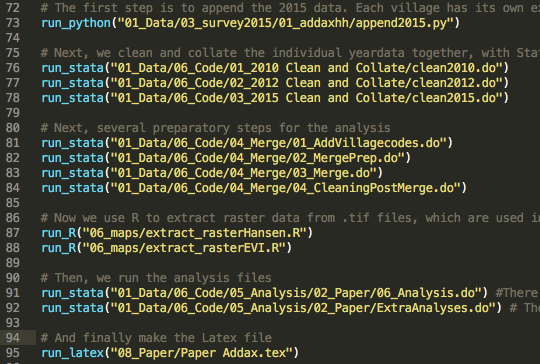
\includegraphics[height=0.8\textheight]{rundirectory_example.png}
\end{frame}

\againframe<2>{howto}

\section{Good Code}

\begin{frame}[t]\frametitle{Good Code}
	\begin{itemize}
		\item We spend a lot of time writing code
		\begin{itemize}
			\item To communicate with the computer: do this
			\item But we also communicate with ourselves: how did I make Figure 2 in research Project X 3 years ago?
		\end{itemize}
		\item Good Code is a necessary skill (or art?) for the modern economist
		\item Guido van Rossum's (Python) key insight: computer code is more often read than written
	\end{itemize}
\end{frame}

\begin{frame}[t]\frametitle{Some Guidelines}
	\begin{itemize}
		\item Be consistent
		\item Readability is more important than succinctness 
		\item Use meaningful but short names
		\begin{itemize}
			\item no:  for i in X 
			\item yes: for var in editvars 
		\end{itemize}
		\item Variable names: lower\_case\_underscores or CamelCase (etc)
		\item Loop as much as you can
		\item Indent in loops and rarely otherwise
		\item Limit line length (80-100 characters)
		\begin{itemize}
			\item To fit two files on one screen
			\item For Github track changes
		\end{itemize}
		\item Write functions for things you do often (more advanced)
	\end{itemize}
\end{frame}

\begin{frame}[t]\frametitle{Commenting}
	\begin{itemize}
		\item `Block comments': brief explanation of next section of code. Always do this
		\item `Inline comments': use sparingly. The code should communicate what happens
		\item But, always comment choices (`Winsorize income at 90\%')
		\item Assume that your reader knows the language (if they don't they shouldn't look at your code)
		\item Be careful: code cannot be out of date, but comments can be. Inconsistency between code and comments is the worst
	\end{itemize}
\end{frame}

\section{Latex}

\begin{frame}[t]\frametitle{Latex}
	\begin{itemize}
		\item Latex is a typesetting system (alternative to Microsoft Word)
		\item Created by Leslie Lamport in 1983
		\item Designed for scientific documenting
		\item Gives you more control over your documents 
		\item Based on the Tex typesetting engine created in 1978 by computer programming legend Donald Knuth 
		\begin{itemize}
			\item Tex is a `finished' product
		\end{itemize}
	\end{itemize}
\end{frame}

\begin{frame}<1>[t, label=adv_latex]\frametitle{Advantages of Latex}
	\begin{itemize}
		\item<1-> Superior typesetting quality
		\item<2-> Equations are easy
		\item<2-> Git can track changes and version history
		\item<3-> Separate writing and typesetting (can reduce distraction)
		\item<3-> Fantastic for scientific presentations
		\item<3-> Great for automation: automatically insert figures and tables
		\item<3-> Good support for citations (BibTex)
		\item<3-> Nerds love it (= Great online support)
		\item<3-> Makes you look smart
	\end{itemize}
\end{frame}

\begin{frame}[t]\frametitle{Typesetting quality}
	\centering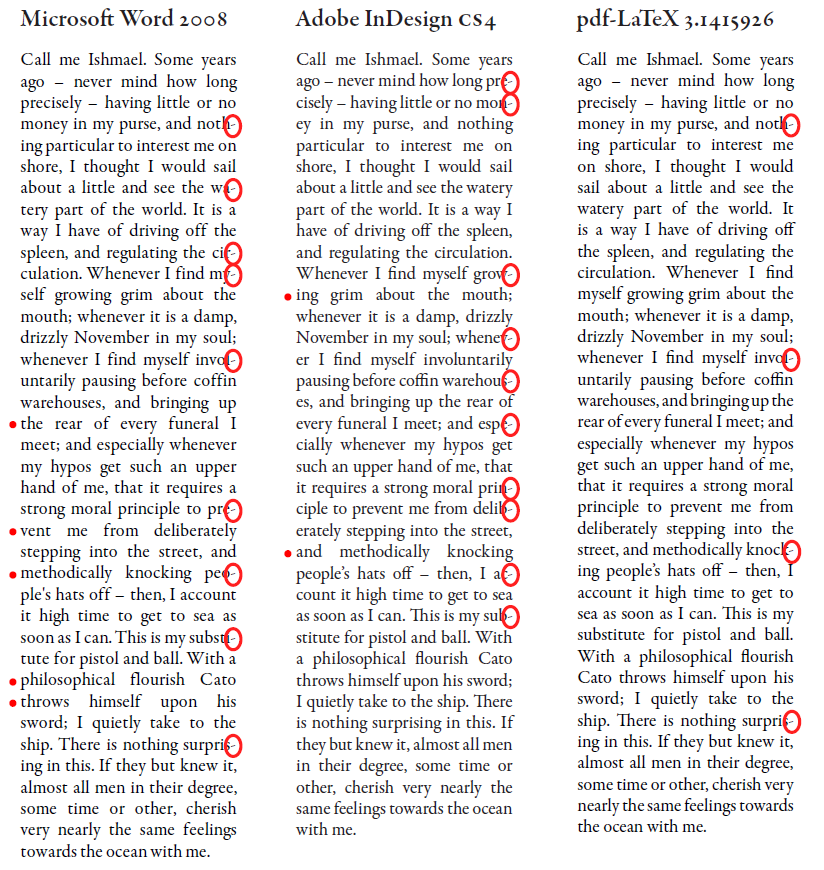
\includegraphics[width=\textwidth]{typesetting_examples.png}
\end{frame}

\begin{frame}[t]\frametitle{Typesetting quality}
	\centering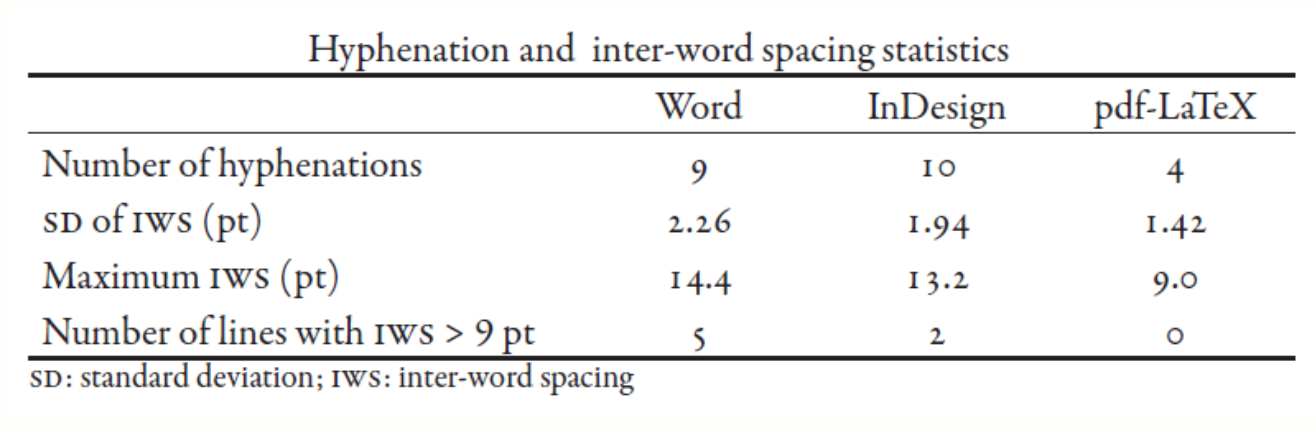
\includegraphics[width=\textwidth]{tex_versus_stats.png}
\end{frame}

\againframe<2>{adv_latex}

\begin{frame}[t]\frametitle{Git and Latex}
	\centering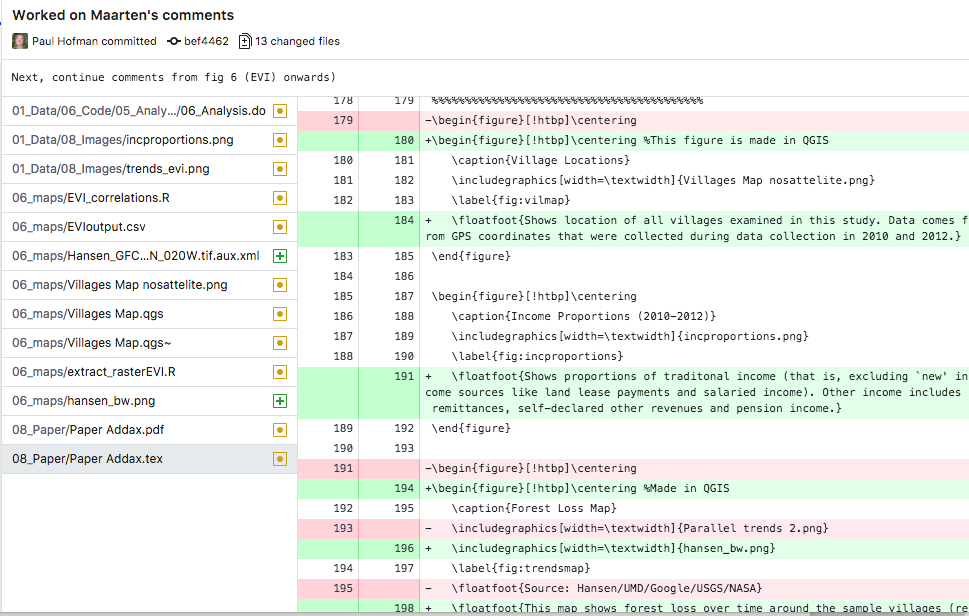
\includegraphics[width=\textwidth]{git_latex_example.png}
\end{frame}

\againframe<3>{adv_latex}

\begin{frame}[t]\frametitle{Disadvantages of Latex}
	\begin{itemize}
		\item Steep learning curve 
		\begin{itemize}
			\item Presentations can be a good introduction
		\end{itemize}
		\item Syntax is cumbersome
		\item Your co-authors don't know how to use it
		\item Word is sometimes a requirement
		\begin{itemize}
			\item There are programs that convert (pandoc)
		\end{itemize}
		\item `Building' your document can take a while
	\end{itemize}
\end{frame}

\begin{frame}[t]\frametitle{Word vs Latex}
	\centering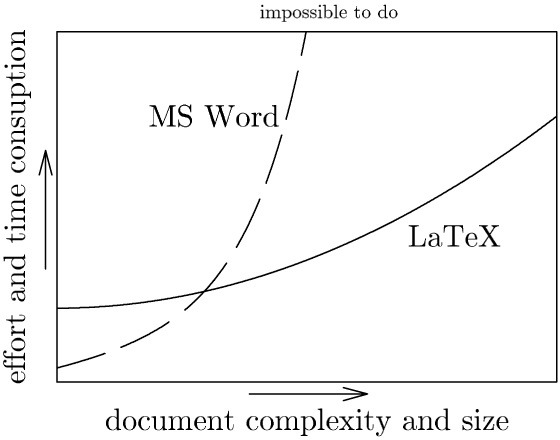
\includegraphics[height=0.8\textheight]{latex_vs_word.jpg}
\end{frame}

\section{R Markdown}

\begin{frame}[t]\frametitle{R Markdown}
	\begin{itemize}
		\item Markdown is a `lightweight' version of Latex: popular for websites (my website uses it)
		\item Created by tech blogger John Gruber in 2004
		\item \textbf{R} Markdown is the statistical suite R, integrated with Markdown
		\item Allows you to import data, run analyses and automatically put them in a table - all in one document
	\end{itemize}
\end{frame}

\begin{frame}[t]\frametitle{R Markdown example}
    \centering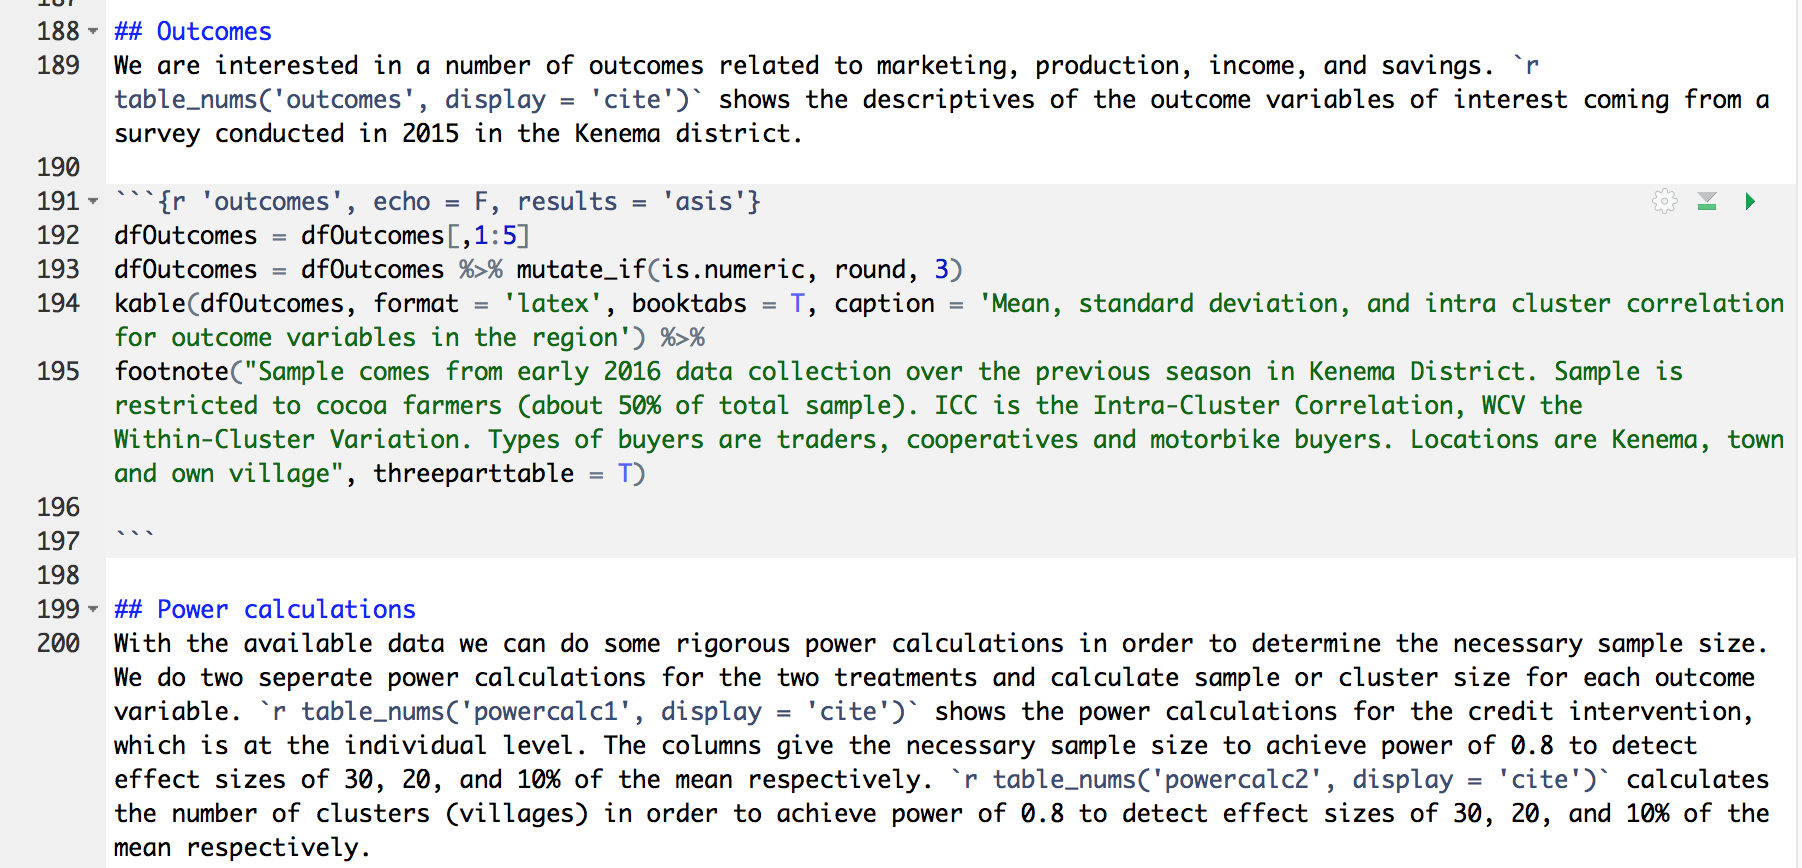
\includegraphics[width=\textwidth]{rmarkdown_example1.png}
\end{frame}

\begin{frame}[t]\frametitle{R Markdown example}
    \centering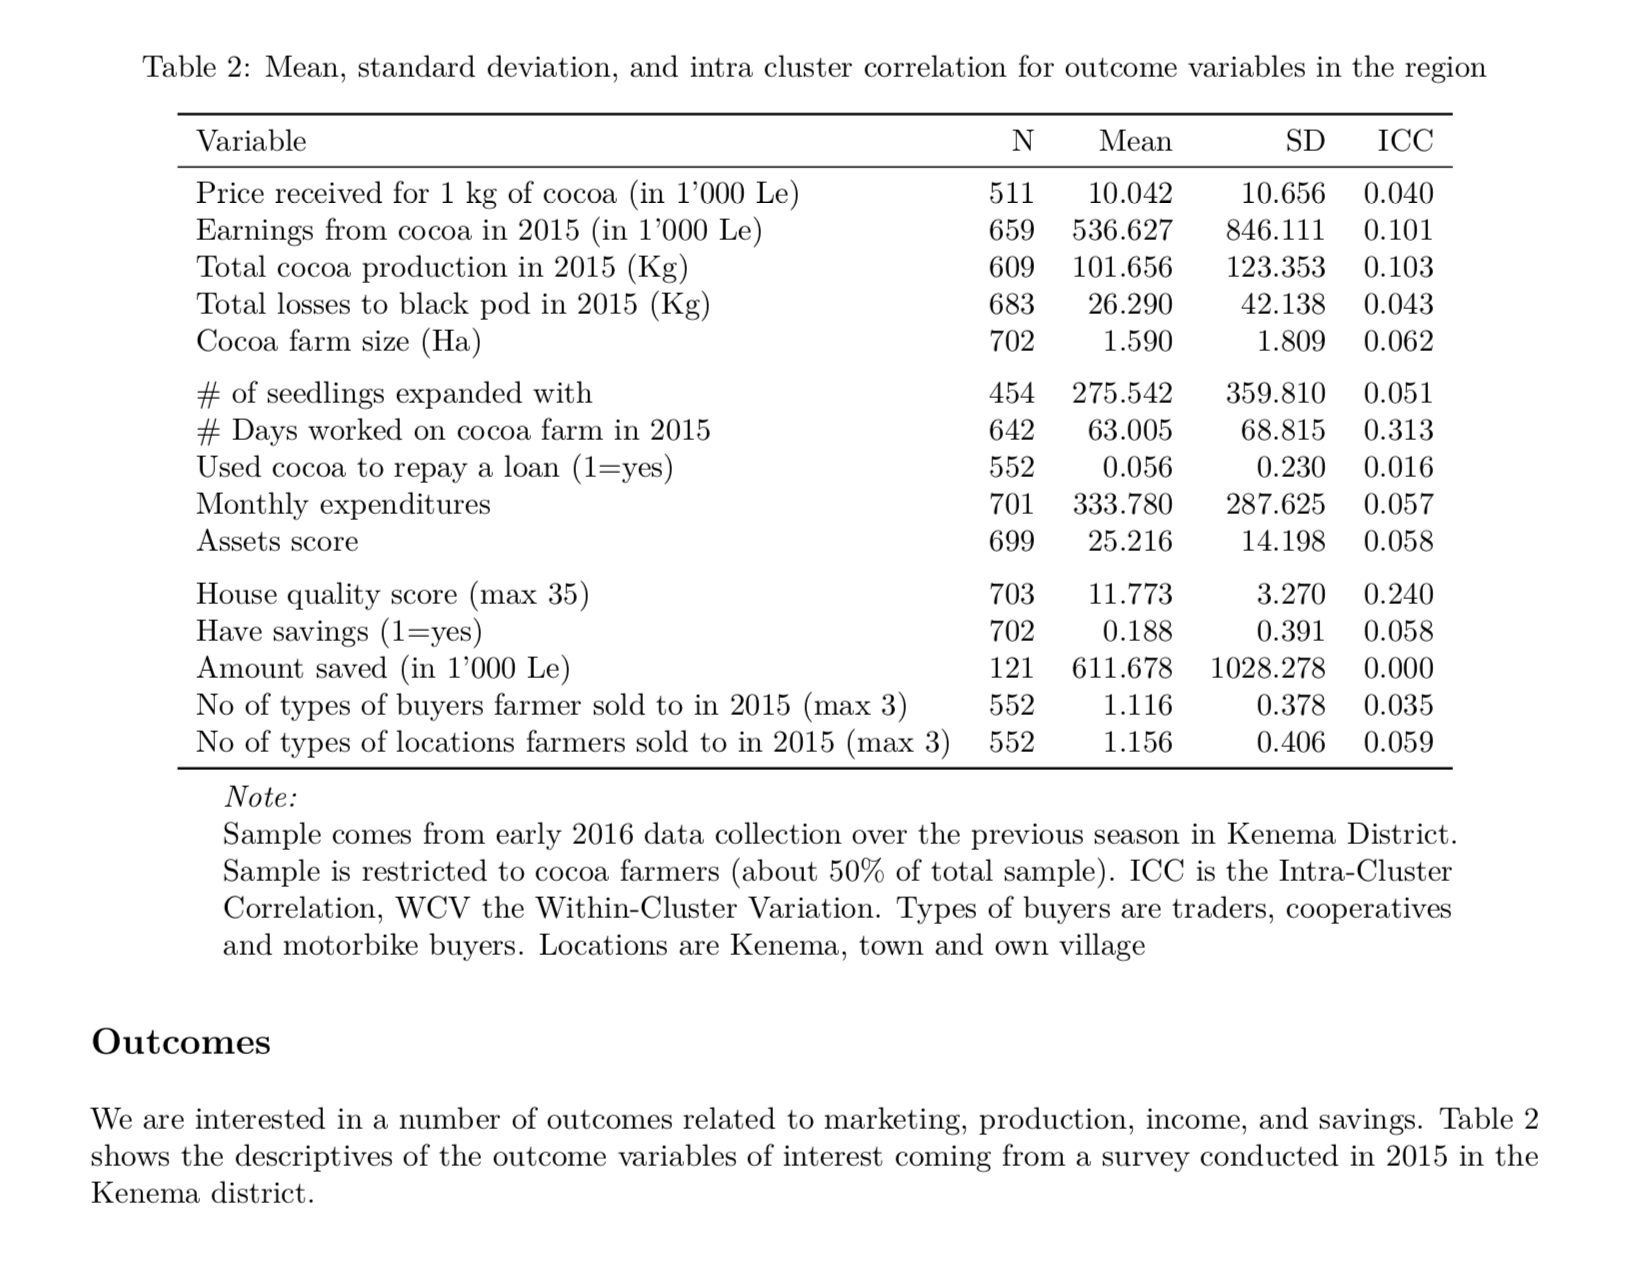
\includegraphics[height=0.8\textheight]{rmarkdown_example2.png}
\end{frame}

\begin{frame}[t]\frametitle{Advantages of R Markdown}
	\begin{itemize}
		\item Very simple syntax
		\item Can include blocks of Latex code for more complicated sections
		\item Your entire paper and the code for analysis in one document
		\item Good support for citations
		\item Fast
	\end{itemize}
\end{frame}

\begin{frame}[t]\frametitle{Disadvantages of R Markdown}
	\begin{itemize}
		\item Only capable of producing simple documents
		\begin{itemize}
			\item Though including Latex sections makes it capable of producing anything
		\end{itemize}
		\item Including code makes the document very long (and a distraction)
		\item Manually making tables is pretty bad
		\item There are different `implementations' of \textit{Markdown}: sometimes uncertain how your document will look
	\end{itemize}
\end{frame}

\section{Workflow}

\begin{frame}[t]\frametitle{Example Workflow}
	Paper that has Python, Stata, R and Latex code \\~\\
	\begin{enumerate}
		\item Raw Data is in appropriate folders, some files downloaded from internet and put in correct folders
		\item Python and Stata clean files
		\item These clean files are picked up by Stata and R to produce analyses tables as .tex files and .png images
		\item These .tex files are picked up by Latex and put in a .pdf
		\item One file, rundirectory.py runs all these scripts in sequence \\~\\
	\end{enumerate}
	Version Control by Github
\end{frame}

\begin{frame}[t]\frametitle{Assorted}
	\begin{itemize}
		\item Use a good Text Editor (Sublime Text, Atom, Textmate)
		\begin{itemize}
			\item I use Sublime Text for R, Latex and Python. Stata maybe soon
		\end{itemize}
	\end{itemize}
\end{frame}

\begin{frame}[t]\frametitle{Further Reading}
	\begin{itemize}
		\item Code and Data for the Social Sciences: A Practitioner's Guide - Matthew Gentzkow and Jesse Shapiro.  \href{http://web.stanford.edu/\~gentzkow/research/CodeAndData.pdf}{Available here} 
		\begin{itemize}
			\item Extremely thorough guide by two economists covering almost all aspects covered here 
		\end{itemize}
		\item How to improve your relationship with your future self -  Jake Bowers and Maarten Voors.  \href{www.revistacienciapolitica.cl/index.php/rcp/article/download/291/22}{Available here} 
		\begin{itemize}
			\item Focuses a lot on writing good code, and R Markdown
		\end{itemize}
		\item PEP8 -- Style guide for python code --  Guido van Rossum   \href{https://legacy.python.org/dev/peps/pep-0008/}{Available here} 
		\begin{itemize}
			\item Really written for Python, but gives great guidelines on coding style
		\end{itemize}
	\end{itemize}
\end{frame}

\end{document}